\documentclass[]{article}
\usepackage{amsmath}
\usepackage{amssymb}
\usepackage{xfrac}
\usepackage[margin=30mm]{geometry}

%opening
\title{Thermodynamic Integration of the Chemical Potential of a 
       Lennard-Jones Fluid}
\author{}

\begin{document}

\maketitle

\begin{abstract}

\end{abstract}

\section*{Introduction}

When performing a Monte Carlo simulation of a system of particles, we compute most desired properties as averages over coordinates in phase space that are generated during the simulation.
Through the Metropolis Method, these calculations depend only on the relative probability of visiting different points in phase space.
We avoid use of absolute probabilities, as this requires a numerical integration over the entire volume in phase space that is accessible to the system, which is simply not feasible.
However, some quantities, such as entropy or free energy, are calculated by integrals over this volume, and so cannot be measured directly in a simulation (or indeed experimentally).
We call these quantities \textit{thermal}.

Thermal quantities may not be directly computable in a simulation, but their derivatives are: for example, for the Helmholz free energy, we have that
\[
	\left.\left(\frac{\partial F}{\partial V}\right)\right\rvert_{N,T} = -P \quad \& \quad \left.\left(\frac{\partial \beta F}{\partial \beta}\right)\right\rvert_{V,N} = E,
\]
and in a Monte Carlo simulation the pressure $P$ and energy $E$ are readily available. 
In this way, if we start from a reference state of known free energy and move it reversibly to the state of interest, we can numerically integrate the change in free energy.
Morover, we are not limited to physical thermodynamic integration paths: any parameter of the potential energy function can be a thermodynamic variable. 

A straightforward way to do this is through Kirkwood's coupling parameter method. 
For an $N$-particle system, we consider a potential energy function
\[
	U:[0,1]\rightarrow \mathbb{R}\quad\mid\quad U(0)=U_{1}, U(1)=U_{2}
\]
where $U_1$ denotes the potential energy of the reference state, and $U_2$ the potential energy of the state of interest.
For each $\lambda$, the partition function of the system is
\[
	Q(N,V,T;\lambda) = (\Lambda^{3N}N!)^{-1}\int e^{-\beta U(\lambda)}d^{3N}x,
\]
and its free energy is $F=-\beta^{-1}\ln Q$. 
This leads us to the expression
\[
	\begin{split}
		\left.\left( \frac{\partial F}{\partial\lambda} \right)\right\rvert_{N,V,T} 
			&= \frac{-1}{\beta}\frac{\partial \ln Q}{\partial\lambda} = \frac{-1}{\beta Q}\frac{\partial Q}{\partial \lambda} \\
			&= \frac{\int\left(\frac{\partial U}{\partial \lambda}\right)e^{-\beta U(\lambda)}\,d^{3N}x}{\int e^{-\beta U(\lambda)}\,d^{3N}x} \\
			&= \left\langle\frac{\partial U}{\partial \lambda}\right\rangle_{\lambda},
	\end{split}
\]
where the ensemble averages are taken using the potential energy function $U(\lambda)$. 
The free energy difference between the reference state $1$ and the state of interest $2$ can be obtained by numerical integration, as we have
\[
	F\rvert_{\lambda=1}-F\rvert_{\lambda=0}=\int_{0}^{1}\left\langle\frac{\partial U}{\partial \lambda}\right\rangle_{\lambda}d\lambda.
\]
This strategy is called thermodynamic integration, and it allows us to express the free energy difference with respect to the reference state in terms of (calculable) ensemble averages.

In practice, a linear interpolation between states $1$ and $2$ is useful. 
This is because the second derivative of $F$ with respect to $\lambda$ is given by
\[
	\begin{split}
		\left.\frac{\partial^2 F}{\partial \lambda^2}\right\rvert_{N,V,T}
			&= -\frac{1}{\beta}\frac{\partial}{\partial\lambda}\left(\frac{\partial_{\lambda}Q}{Q}\right) 
				= \frac{-1}{\beta}\frac{Q\partial^{2}_\lambda Q - (\partial_{\lambda}Q)^2}{Q^2} 
				= \frac{-1}{\beta Q}\frac{\partial^2 Q}{\partial \lambda^2} + \beta\left[\frac{-1}{\beta Q}\frac{\partial Q}{\partial \lambda}\right]^2\\
			&= -\beta\left[ \left\langle\left(\frac{\partial U}{\partial \lambda}\right)^2\right\rangle_{\lambda} 
				- \left\langle\frac{\partial U}{\partial \lambda}\right\rangle^{2}_{\lambda} 
				- \beta^{-1} \left\langle\frac{\partial^2 U}{\partial \lambda^2}\right\rangle_{\lambda}\right].
	\end{split}
\]
If we take 
\[
	U(\lambda) = U_{1} + \lambda(U_{2}-U_{1}),
\]
the third term vanishes, and we immediately obtain the Gibb-Bogoliubov inequality
\[
	\left.\frac{\partial^2 F}{\partial \lambda^2}\right\rvert_{N,V,T} = -\beta\left[\left\langle(U_2-U_1)^2\right\rangle_{\lambda}-\left\langle U_2-U_1 \right\rangle^{2}_{\lambda}\right]\leq 0.
\]
This implies that $\frac{\partial F}{\partial \lambda}$ cannot increase with $\lambda$, which is useful to verify against simulation results.
\section*{Methods}

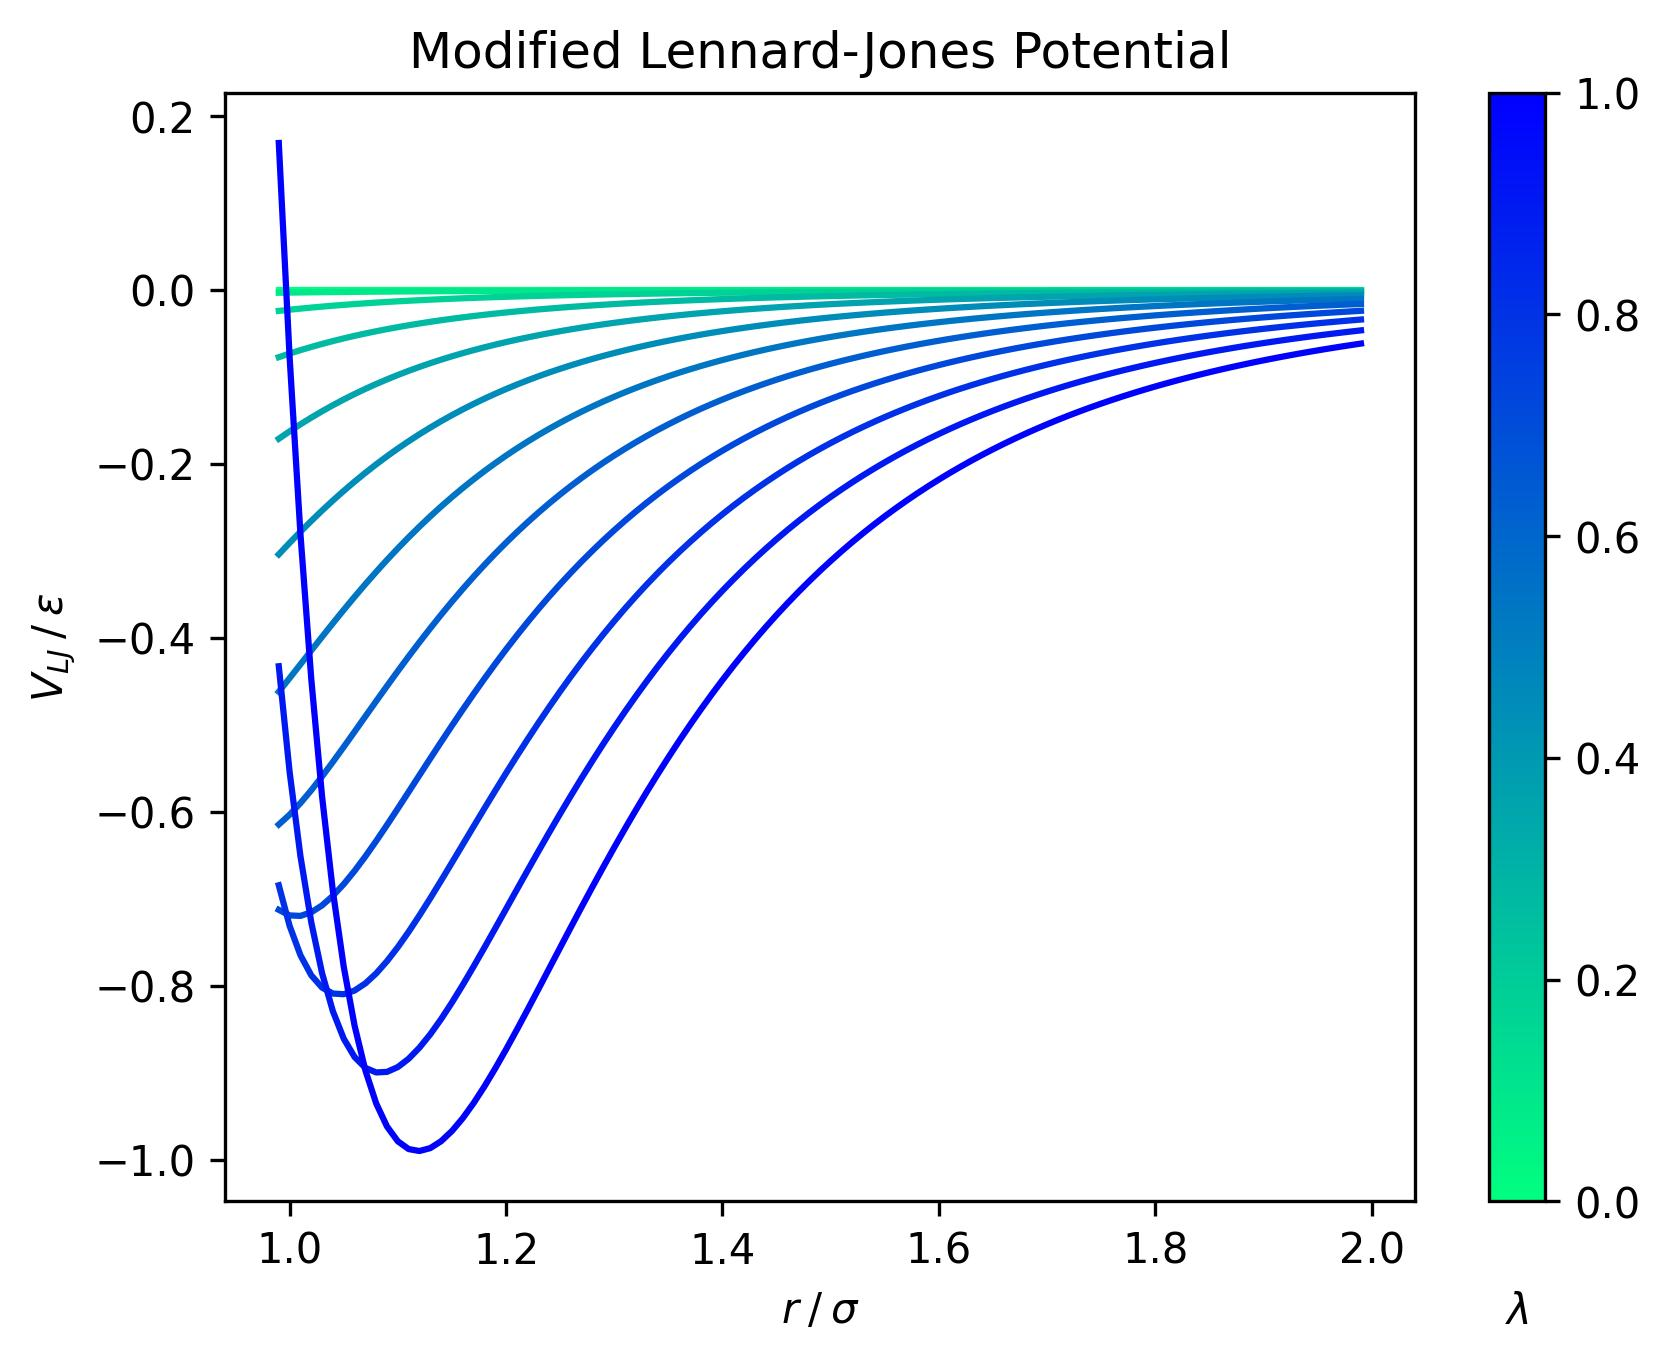
\includegraphics[width=0.5\linewidth]{modLJ.jpg}

\section*{Results}

\section*{Conclusions}

\end{document}
